% =====================================================================
%  Figure panels for: Mekaneck -- A Substrate-Neutral Language
%  Captions quote measured values; see validation/results/panel_stats.json
% =====================================================================

\begin{figure*}[!htbp]
    \centering
    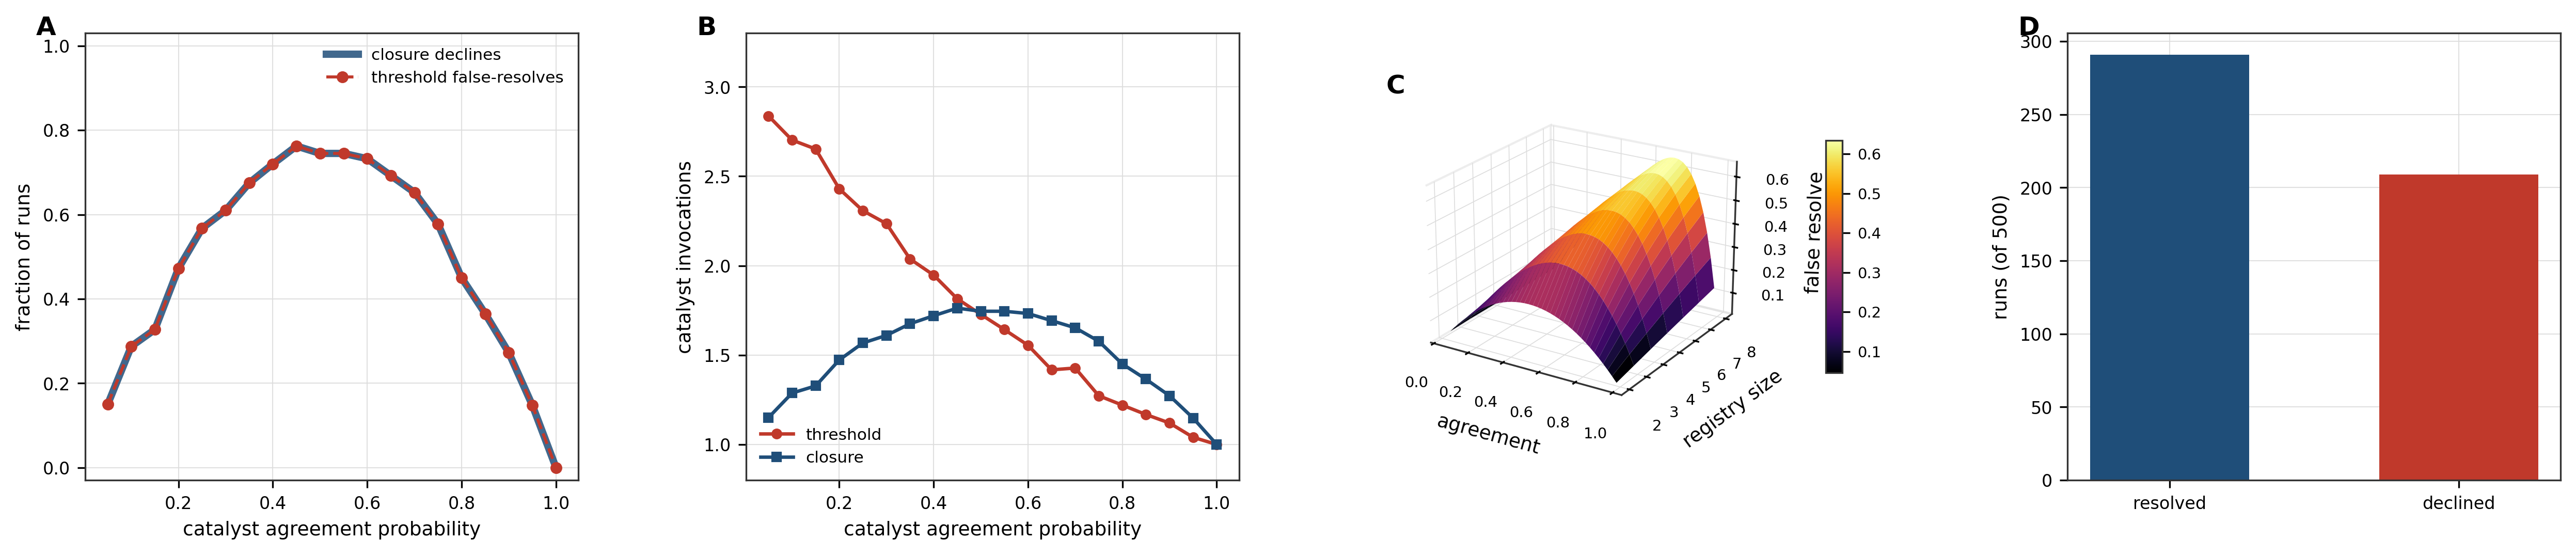
\includegraphics[width=\textwidth]{figures/panel-1-closure.png}
    \caption{\textbf{A threshold rule fails on exactly the runs where the evidence is contested, and the two rates coincide identically rather than approximately.}
    Every point is measured by evaluating the same \texttt{seek} under the two termination rules on identical substrates and identical catalyst orderings, so the comparison isolates the stopping criterion and nothing else. The confident cell carries attained uncertainty $5.0$ against a threshold of $10.0$; the incompatible alternative carries $40.0$ and never satisfies the threshold alone.
    (\textbf{A})~Fraction of runs on which closure declines, and fraction on which the threshold rule reports a single answer despite the evidence being split, against the probability that catalysts agree; $400$ substrates at each of $20$ levels. The two curves are equal to machine precision at every level---maximum absolute difference $0.0$---which is why one is drawn heavy and the other dashed over it. The coincidence is not a coefficient to be estimated: whenever the reachable set contains more than one cell, some catalyst reaches the cell satisfying the threshold, and the threshold rule halts there by construction. On this substrate family the threshold rule is wrong on every contested run and on no others. The rate is non-monotone, peaking at $0.763$ near even agreement and falling to $0.150$ and $0.0$ at the extremes, because unanimity---on either cell---leaves nothing contested.
    (\textbf{B})~Catalyst invocations paid by each rule. The threshold rule pays $2.84$ invocations when agreement is low and $1.0$ when it is high; closure peaks at $1.76$ in the middle. The threshold rule is therefore cheapest exactly where it errs most, which is the economic shape of the failure mode: it stops early precisely when stopping early is unsafe.
    (\textbf{C})~False-resolve rate over agreement probability and registry size. The surface rises with registry size at fixed agreement, because each additional uninvoked catalyst is a further opportunity for an unconsulted source to disagree. Enlarging the registry---adding evidence---makes a threshold rule worse, which inverts the relationship an inquiry should have with its own resources.
    (\textbf{D})~Outcome split over $500$ random substrates: $291$ resolved, $209$ declined. Both branches of \Cref{thm:dichotomy} occur under ordinary substrate sampling. We report the split because a dichotomy theorem is compatible with one branch being unreachable in practice, and a language whose declination branch never fired would be a threshold rule wearing different syntax.}
    \label{fig:mpanel1}
\end{figure*}

\begin{figure*}[!htbp]
    \centering
    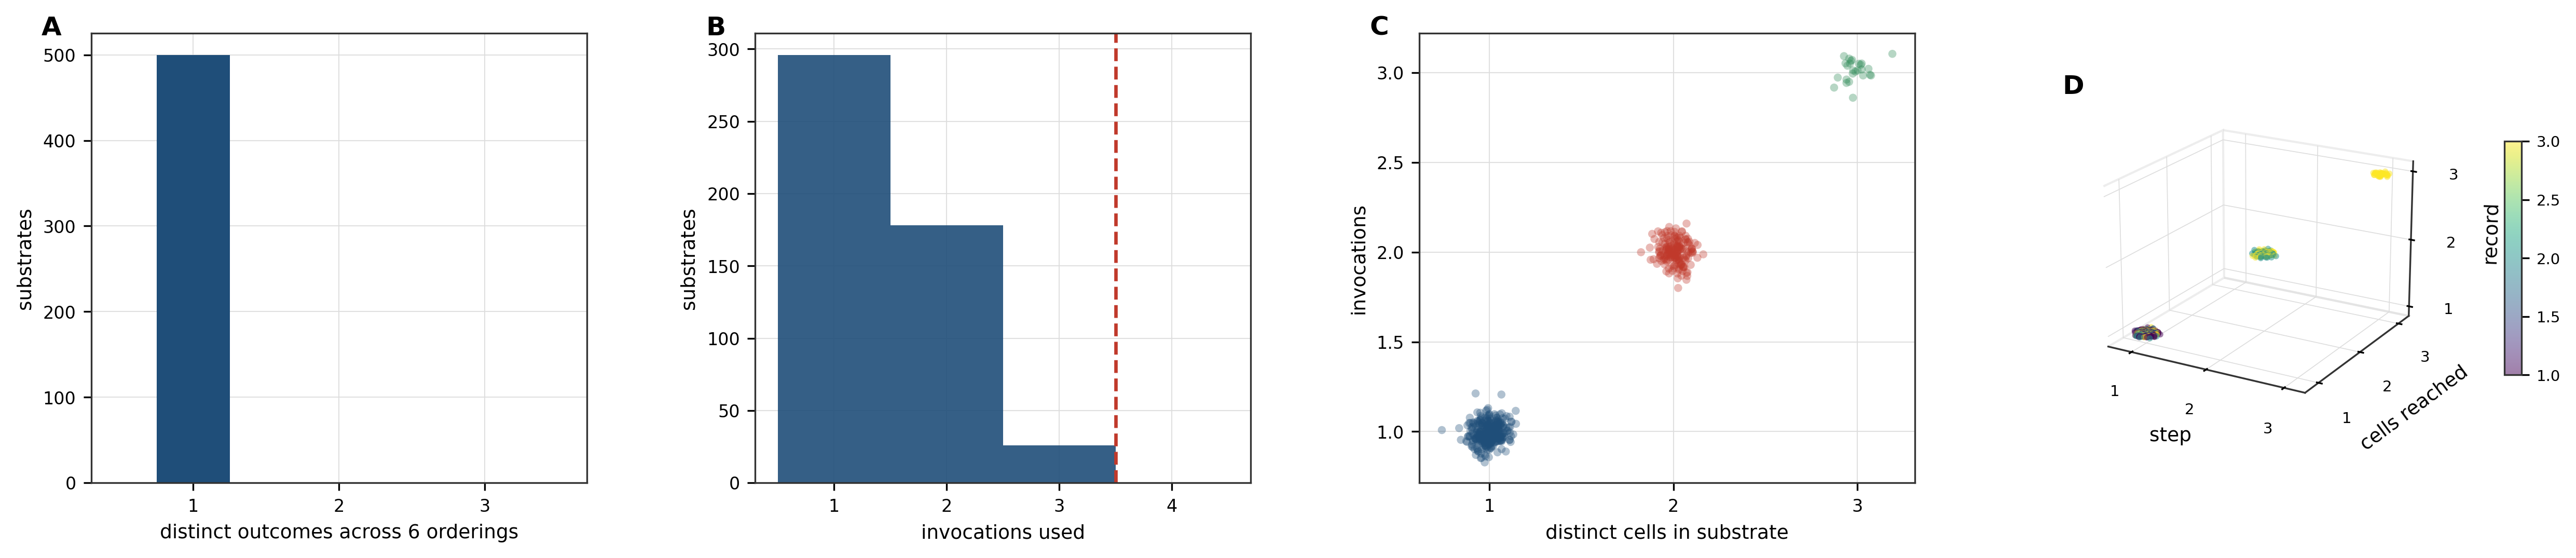
\includegraphics[width=\textwidth]{figures/panel-2-semantics.png}
    \caption{\textbf{The metatheory holds on every evaluation tested, and the invocation count is exactly the number of destinations the substrate contains.}
    $500$ random substrates, each evaluated under all six orderings of the catalyst set---$3000$ evaluations---with outcomes compared by structural equality rather than by representative.
    (\textbf{A})~Distinct outcomes obtained across the six orderings, per substrate. Every substrate yields exactly one: there are no substrates in the two- or three-outcome bins. This is \Cref{thm:determinism}, and it holds because the reached-cell set is built by union, which is order-insensitive, while the closure rules branch only on that set's cardinality. Non-determinism can therefore enter only through the substrate's own responses, never through the language.
    (\textbf{B})~Invocations used per substrate against the bound $\abs{\Env_{\mathrm{avail}}}=3$ marked in red. The distribution is supported entirely at or below the bound---$296$ substrates at one invocation, $178$ at two, $26$ at three, none above---confirming \Cref{thm:termination} with no exceptions. The strong skew toward a single invocation shows that closure is usually cheap: it costs the full registry only when the registry genuinely disagrees.
    (\textbf{C})~Invocations against the number of distinct cells the substrate contains. The two are equal on every substrate, giving three tight clusters on the diagonal with no off-diagonal mass. A \texttt{seek} therefore invokes exactly as many catalysts as there are distinct destinations to discover and stops---it does not exhaust the registry when the registry agrees, and does not stop early when it does not.
    (\textbf{D})~Record against step and cells reached, over every ordering of every substrate, coloured by the substrate's cell count. Points lie only where record equals step, so each committed invocation advances the record by exactly one, and the cells-reached coordinate is non-decreasing along every trajectory. No configuration recurs at a smaller record, which is \Cref{thm:monotone}: a program's provenance ordering is intrinsic to its own execution and needs no external timestamp.}
    \label{fig:mpanel2}
\end{figure*}

\begin{figure*}[!htbp]
    \centering
    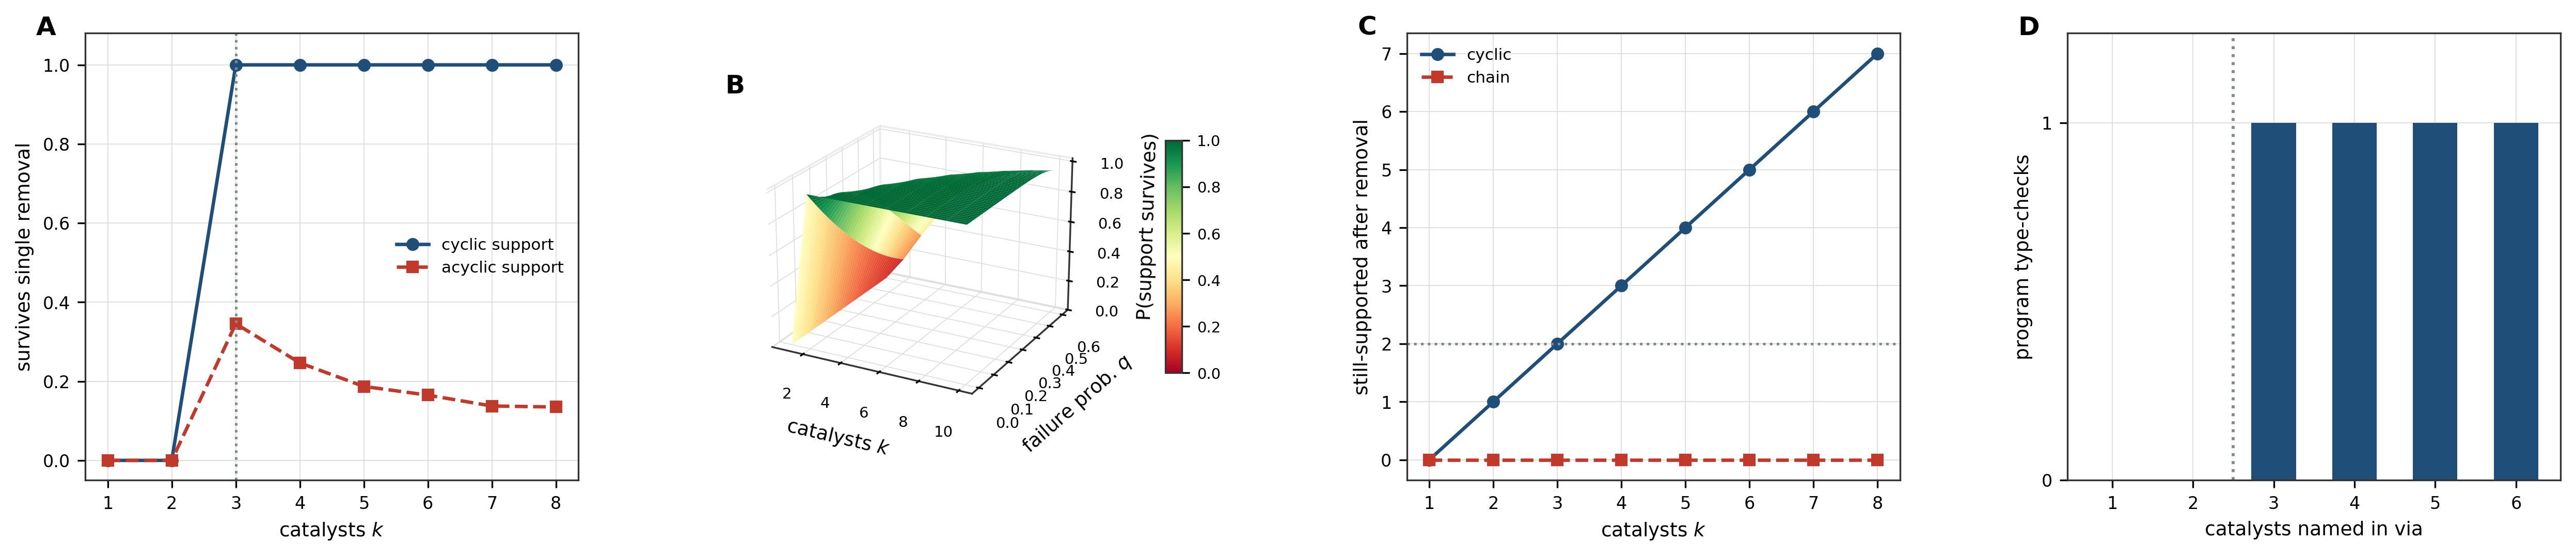
\includegraphics[width=\textwidth]{figures/panel-3-coherence.png}
    \caption{\textbf{Robustness against the loss of a single source appears at three catalysts and not before, and the type checker enforces the boundary rather than recommending it.}
    Panels (A)--(C) evaluate the combinatorics of support structures; panel (D) is measured from the implementation, by submitting programs to the type checker and recording what it accepts.
    (\textbf{A})~Probability that a conclusion survives removal of an arbitrary single catalyst, for cyclic and acyclic support structures, against the number of catalysts. Cyclic support jumps from $0$ at $k=2$ to $1$ at $k=3$ and stays there; acyclic support peaks at $0.34$ and decays toward zero, never reaching robustness at any size. This is \Cref{thm:linear} and \Cref{thm:three} together: no chain is robust however long, because its terminal member is licensed by nothing, and the shortest cycle compatible with robustness has length three. A $2$-cycle fails not for want of evidence but for want of an arbiter---removing either member leaves the other supported by nothing.
    (\textbf{B})~Probability that at least two mutually supporting catalysts remain after independent per-catalyst failures, over $k$ and the failure probability $q$. At $q=0.2$ the probability rises from $0.640$ at $k=2$ to $0.896$ at $k=3$ and $0.993$ at $k=5$; at $q=0.4$ the same $k=3$ structure retains only $0.648$. The third catalyst is the step that lifts the surface away from the failure plane, and the surface makes visible what the rule cannot promise: three unreliable catalysts are not equivalent to three reliable ones, and the rule constrains structure, not quality.
    (\textbf{C})~Number of catalysts still supported after one removal. A cycle retains $k-1$, rising linearly; a chain retains none at any $k$. The dotted line at two marks the minimum needed for mutual support to persist, which the cyclic case first clears at $k=3$.
    (\textbf{D})~Whether the type checker accepts a program naming $k$ mutually independent catalysts. Programs at $k=1$ and $k=2$ are rejected by \textsc{T-Seek-Coh}; programs at $k=3$ through $6$ are accepted. The boundary is enforced at compile time and is not a convention a user may set aside. What the rule cannot do is verify the independence it requires (\Cref{rem:coh-limits}): three catalysts sharing an upstream data source or a common preprocessing step satisfy it while violating its intent, so the declaration is made visible in the source and left auditable rather than checked.}
    \label{fig:mpanel3}
\end{figure*}

\begin{figure*}[!htbp]
    \centering
    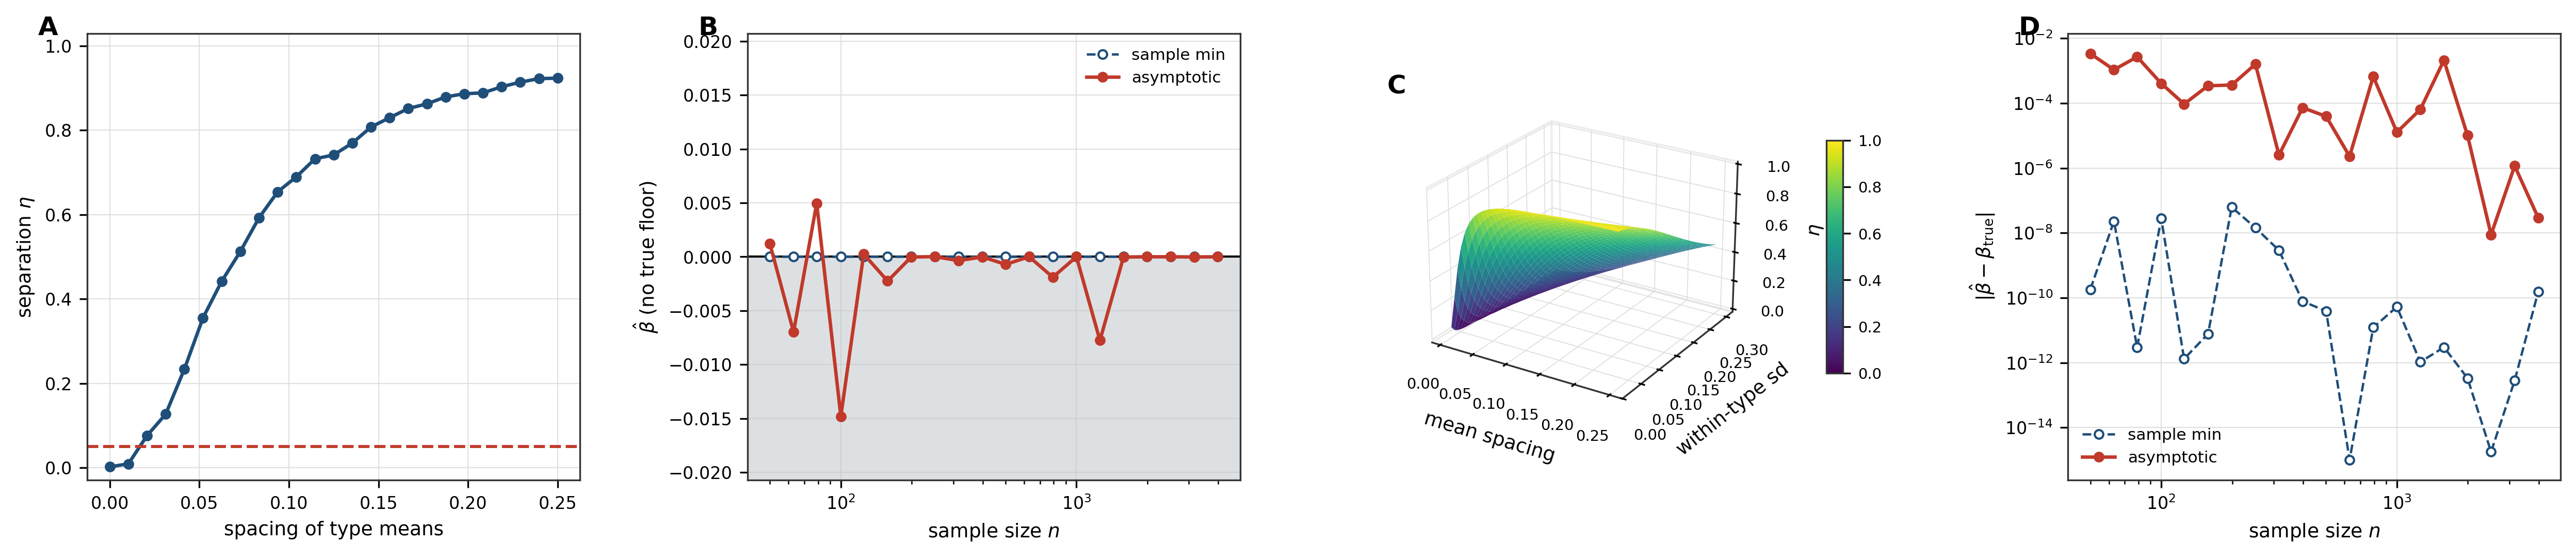
\includegraphics[width=\textwidth]{figures/panel-4-diagnostics.png}
    \caption{\textbf{Two diagnostics the type system cannot supply: whether a binding's events discriminate, and whether its floor obligation was discharged by an estimator capable of failing.}
    The language depends on a substrate only through the four obligations of \Cref{def:substrate} and cannot inspect what discharges them. These charts are the instruments a substrate author is asked to run instead.
    (\textbf{A})~Separation $\eta$ as the event types' mean powers are drawn together, with the flagging threshold at $0.05$. Separation falls from $0.924$ at wide spacing to $1.8\times10^{-3}$ when the means coincide, crossing the threshold at a spacing of about $0.010$. Below the line the per-type means are indistinguishable, predictions formed from them are constant at fixed cascade length, and no comparison among composition rules has discriminating power. A negative result obtained in this region is evidence about the observable, not about the process (\Cref{prop:uninformative}), and should be reported as an uninformative binding rather than as a disconfirmation.
    (\textbf{B})~Signed floor estimate on a process with \emph{no} floor, $20$ sample sizes. The sample minimum is strictly positive at every one, never falling below $3.2\times10^{-13}$ and never reaching zero; the asymptotic intercept is negative at $12$ of the $20$, reaching $-1.5\times10^{-2}$. The shaded band is the region an observation must enter to contradict a positivity claim. An estimator bounded below by zero cannot enter it, so a substrate discharging obligation~(S4) by returning a sample minimum has made a claim no data could refute (\Cref{rem:floor-diag}). This is why a binding is required to declare its estimator in the source.
    (\textbf{C})~$\eta$ over the spacing of type means and the within-type dispersion. Separation is governed by the ratio of the two rather than by either alone, so the contour lines are radial: a substrate that fails the diagnostic can be rescued either by sharpening its observable, which widens the spacing, or by refining its typing, which narrows the dispersion. The surface tells an author which of the two is the cheaper fix for their binding.
    (\textbf{D})~Absolute error of both estimators against sample size on a process whose true floor is $10$, log--log axes. Both converge and the sample minimum is the more accurate throughout, which we record because it cuts against the recommendation: accuracy on a floored process is not the property at issue. Panel~(B) is, and there the two estimators differ in kind rather than in degree.}
    \label{fig:mpanel4}
\end{figure*}
